\section{CI / CD}

\frame{\tableofcontents[currentsection]}

\begin{frame}
    \frametitle{What is Continuous Integration?}   
    \begin{itemize}
        \item \href{https://circleci.com/blog/what-is-continuous-integration/}{[BLOG POST]}
        \item multiple developers pushing small, frequent changes to a shared repository
        \item \href{https://en.wikipedia.org/wiki/Continuous_integration}{[COMMON PRACTICES]}
        \item often comes with Continuous Deployment
        \item CircleCI build has generally multiple steps:
        \begin{itemize}
            \item dependencies
            \item testing
            \item deployment
        \end{itemize}
    \end{itemize}
\end{frame}

\begin{frame}
    \frametitle{How your repo will look like}   
    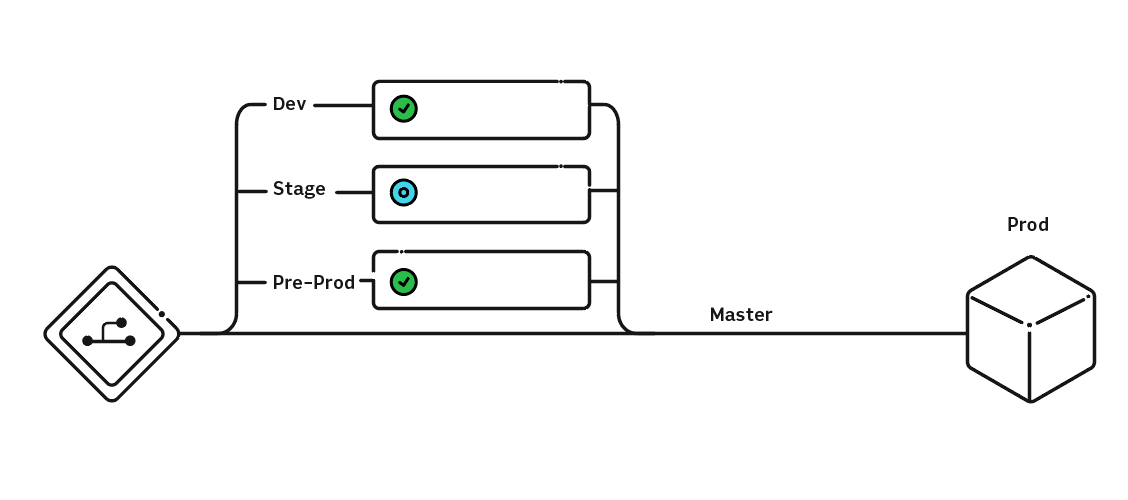
\includegraphics[scale=0.25]{01-sample-branches}
    
    feel free to simplify this to following branches:
    \begin{itemize}
        \item dev
        \item prod
    \end{itemize}
    you can configure your CI/CD to do specific task on specific branches (e.g. only deploy prod branch)
\end{frame}

\begin{frame}
    \frametitle{Github repo demo}   
\end{frame}

\begin{frame}
    \frametitle{Demo steps}   
    \begin{itemize}
        \item create github repo with default generated project
        \item Log in to CircleCI
        \item On the left pane, click add project
        \item Click "set up project"
        \item Do not use the sample config.yml
        \item in your root folder, create a ".circleci" folder with the file "config.yml"
        \item use the following file: \href{https://circleci.com/docs/2.0/language-elixir/}{[LINK]}
        \item adjust circleci config to mysql
        \item adjust mysql root password in test environment config
        \item adjust junit formatter
    \end{itemize}
\end{frame}


\begin{frame}
    \frametitle{Demo steps}   
    \begin{itemize}
        \item add create test report folder step BEFORE mix test
        \item add artifact step
        \item badge
        \item for badge create token
        \item then create badge
    \end{itemize}
\end{frame}
